\documentclass[12pt, a4paper]{article}

\usepackage[
  margin=1in
]{geometry}

\usepackage[T1, T2A]{fontenc}
\usepackage[utf8]{inputenc}
\usepackage[russian]{babel}
\usepackage{minted}
\usepackage{tabularray}
\usepackage{siunitx}
\usepackage{graphicx}

\graphicspath{ {./img/} }

\begin{document}

\begin{titlepage}
  \centering
  \textsc{Новосибирский государственный технический университет}\par
  \vspace{1mm}
  Кафедра прикладной математики\par
  \vspace{4cm}
  \textsc{Практическая работа \textnumero 2}\par
  {\huge\bfseries Параллельные операции с векторами и матрицами на OpenMP\par}
  \vspace{1cm}
  {\scriptsize ФПМИ, ПМ-24\par}
  \vspace{1mm}
  {\itshape\large Параскун И., Шакиров П., Герасименко В.\par}
  \vfill
  {\small преподаватель\par}
  \vspace{1mm}
  \textsc{Домников Петр Александрович}
  \vfill
  \large{Новосибирск, 2024}
\end{titlepage}

\newpage
\setcounter{page}{2}

\section{Умножение векторов}
\subsection{Постановка задачи}
Написать программу параллельного вычисления скалярного произведения:

$$ (x, y) = \sum_{i=1}^{n} x_iy_i $$

\noindent Протестировать ее на векторе малого размера. Сравнить результат и время выполнения программы последовательной
и параллельной версий.

\subsection{Текст программы}

\begin{minted}{c}
void vec_mlt(struct vec* a, struct vec* b, real* r) {
  real s = 0;

#pragma omp parallel for reduction(+ : s) num_threads(THRD)
  for (size_t i = 0; i < a->n; ++i)
    s += a->v[i] * b->v[i];

  *r = s;
}
\end{minted}
\textit{*вычислительная функция}

\begin{minted}{c}
int main(int argc, char* argv[argc]) {
  struct timespec s;
  struct timespec e;

  struct vec* a = vec_seq(N);
  struct vec* b = vec_seq(N);

  real prod;

  clock_gettime(CLOCK_MONOTONIC_RAW, &s);
  vec_mlt(a, b, &prod);
  clock_gettime(CLOCK_MONOTONIC_RAW, &e);

  printf("Product: %.1lf\n", prod);
  printf("Execution time: %.3e ms.\n", to_ms(&s, &e));

  return 0;
}
\end{minted}
\textit{*вызывающая подпрограмма}

\begin{minted}{console}
[mehandes@neptune build]$ ./algo
Product: 5.0
Execution time: 1.373e-03 ms.
\end{minted}
\textit{*результат выполнения при малой размерности векторов (3)}

\newpage
\subsection{Результат выполнения}

\begin{table}[ht]
\centering
\begin{tblr}{
  width=\textwidth, 
  colspec={|l|X|X|X|X|},
  rowspec={|c|c|ll|}
}
\SetCell[r=2]{c} $N$  & \SetCell[c=4]{c} Dot product                                    & & & \\
                      & 1               & 2               & 6               & 12              \\
1E+03                 & 332833500.0     & 332833500.0     & 332833500.0     & 332833500.0     \\
1E+05                 & 12***.0         & 12***.0         & 12.***.0        & 12.***.0        \\
\end{tblr}
\end{table}

\begin{table}[ht]
\centering
\begin{tblr}{
  width=\textwidth, 
  colspec={|l|X|X|X|X|},
  rowspec={|c|c|llll|}
}
\SetCell[r=2]{c} $N$  & \SetCell[c=4]{c} Time, ms                   & & & \\
                      & 1         & 2         & 6         & 12            \\
1E+03                 & 7.424E-03 & 6.522E-03 & 5.190E-03 & 9.267E-01     \\
1E+05                 & 7.339E-01 & 3.821E-01 & 1.779E-01 & 8.118E-02     \\
1E+07                 & 2.891E+01 & 1.451E+01 & 5.991E+00 & 5.776E+00     \\
1E+09                 & 1.627E+04 & 2.000E+04 & 6.739E+03 & 4.333E+03     \\
\end{tblr}
\end{table}

\begin{table}[ht]
\centering
\begin{tblr}{
  width=\textwidth, 
  colspec={|l|X|X|X|X|},
  rowspec={|c|c|llll|}
}
\SetCell[r=2]{c} $N$  & \SetCell[c=4]{c} Acceleration               & & & \\
                      & 1         & 2         & 6         & 12            \\
1E+03                 & 1.000E+00 & 1.138E+00 & 1.430E+00 & 8.011E-03     \\
1E+05                 & 1.000E+00 & 1.921E+00 & 4.125E+00 & 9.040E+00     \\
1E+07                 & 1.000E+00 & 1.992E+00 & 4.826E+00 & 5.005E+00     \\
1E+09                 & 1.000E+00 & 8.135E-01 & 2.414E+00 & 3.755E+00     \\
\end{tblr}
\end{table}

\newpage
\section{Умножение матриц}
\subsection{Постановка задачи}
Написать параллельную программу умножения матриц:

$$ C = AB $$

\noindentВычислить норму полученной матрицы:

$$ ||C||=\sqrt{\sum_{i,j}c_{ij}^2} $$

\noindentСравнить норму и время выполнения последоватной и параллельной версий программы.

\subsection{Текст программы}
\begin{minted}{c}
void mtx_mmlt(struct mtx* a, struct mtx* b, struct mtx* c) {
#pragma omp parallel for num_threads(THRD)
  for (size_t i = 0; i < a->n; ++i)
    for (size_t j = 0; j < a->n; ++j) {
      c->v[i * a->n + j] = 0.0;

      for (size_t e = 0; e < a->n; ++e)
        c->v[i * a->n + j] += a->v[i * a->n + e] * b->v[e * a->n + j];
    }
}

void mtx_norm(struct mtx* a, real* r) {
  for (size_t i = 0; i < a->n; ++i)
    for (size_t j = 0; j < a->n; ++j)
      *r += a->v[i * a->n + j] * a->v[i * a->n + j];

  *r = sqrt(*r);
}
\end{minted}
\textit{*вычислительные функции}

\begin{minted}{c}
int main(int argc, char* argv[argc]) {
  struct timespec s;
  struct timespec e;

  struct mtx* a = mtx_seq(N);
  struct mtx* b = mtx_seq(N);
  struct mtx* c = mtx_new(N);

  real norm;

  clock_gettime(CLOCK_MONOTONIC_RAW, &s);
  mtx_mmlt(a, b, c);
  clock_gettime(CLOCK_MONOTONIC_RAW, &e);

  mtx_norm(c, &norm);

  printf("Norm: %.7lf\n", norm);
  printf("Execution time: %.3e ms.\n", to_ms(&s, &e));

  return 0;
}
\end{minted}
\textit{*вызывающая подпрограмма}

\begin{minted}{console}
[mehandes@neptune build]$ ./algo 
***.00e+00***.000e+00***.000e+00 
***.00e+00***.000e+00***.000e+00 
***.00e+00***.000e+00***.000e+00 

***.00e+00***.000e+00***.000e+00 
***.00e+00***.000e+00***.000e+00 
***.00e+00***.000e+00***.000e+00 

***.00e+00***.000e+00***.000e+00 
***.00e+00***.000e+00***.000e+00 
***.00e+00***.000e+00***.000e+00 

Norm: 11.6189500
Execution time: 1.052e-03 ms.
\end{minted}
\textit{*результат выполнения при малой размерности матриц}

\newpage
\subsection{Результат выполнения}

\begin{table}[ht]
\centering
\begin{tblr}{
  width=\textwidth, 
  colspec={|l|X|X|X|X|},
  rowspec={|c|c|llll|}
}
\SetCell[r=2]{c} $N$  & \SetCell[c=4]{c} Norm                                   & & & \\
                      & 1             & 2             & 6             & 12            \\
1.0E+03               & 288170***.*** & 288170***.*** & 288170***.*** & 288170***.*** \\
1.5E+03               & 145971***.*** & 145971***.*** & 145971***.*** & 145971***.*** \\
2.0E+03               & 461476***.*** & 461476***.*** & 461476***.*** & 461476***.*** \\
2.5E+03               & 112684***.*** & 112684***.*** & 112684***.*** & 112684***.*** \\
\end{tblr}
\end{table}

\begin{table}[ht]
\centering
\begin{tblr}{
  width=\textwidth, 
  colspec={|l|X|X|X|X|},
  rowspec={|c|c|llll|}
}
\SetCell[r=2]{c} $N$    & \SetCell[c=4]{c} Time, ms                   & & & \\
                        & 1         & 2         & 6         & 12            \\
1.0E+03                 & 5.386E+03 & 2.763E+03 & 9.907E+02 & 8.071E+02     \\
1.5E+03                 & 3.020E+04 & 1.485E+04 & 4.047E+03 & 2.794E+03     \\
2.0E+03                 & 6.495E+04 & 3.206E+04 & 9.533E+03 & 6.792E+03     \\
2.5E+03                 & 1.398E+05 & 6.758E+04 & 1.815E+04 & 1.405E+04     \\
\end{tblr}
\end{table}

\begin{table}[ht]
\centering
\begin{tblr}{
  width=\textwidth, 
  colspec={|l|X|X|X|X|},
  rowspec={|c|c|llll|}
}
\SetCell[r=2]{c} $N$  & \SetCell[c=4]{c} Acceleration               & & & \\
                      & 1         & 2         & 6         & 12            \\
1E+03                 & 1.000E+00 & 1.949E+00 & 5.437E+00 & 6.673E+00     \\
1E+05                 & 1.000E+00 & 2.034E+00 & 7.462E+00 & 1.081E+01     \\
1E+07                 & 1.000E+00 & 2.026E+00 & 6.813E+00 & 9.563E+00     \\
1E+09                 & 1.000E+00 & 2.069E+00 & 7.702E+00 & 9.950E+00     \\
\end{tblr}
\end{table}

\newpage
\section{Решение СЛАУ}
\subsection{Постановка задачи}

Написать параллельную программу для решения систем линейных алгебраических уравнений:

$$ Ux = b $$

\noindentгде $U$ - известная верхетреугольная матрица.
\vspace{2mm}
\par\noindentПо заданному вектору $x$ найти вектор $b$, используя
параллельный алгоритм умножения матрицы на вектор.
\vspace{2mm}
\par\noindentРешить систему:

$$ Uy = b $$

\noindentСравнить полученный вектор $y$ и исходный вектор $x$. 
Сравнить их нормы.

\subsection{Текст программы}
\begin{minted}{c}
void sle_gauss(struct mtx* a, struct vec* x, struct vec* b) {
  for (int i = a->n - 1; i >= 0; --i) {
    real xi = b->v[i];

#pragma omp parallel for reduction(- : xi) num_threads(TN)
    for (size_t j = i + 1; j < a->n; ++j)
      xi -= x->v[j] * a->v[i * a->n + j];

    x->v[i] = x->v[i] / a->v[i * a->n + i];
  }
}

void mtx_vmlt(struct mtx* a, struct vec* b, struct vec* c) {
#pragma omp parallel for num_threads(THRD)
  for (size_t i = 0; i < a->n; ++i) {
    c->v[i] = 0.0;

    for (size_t j = 0; j < a->n; ++j)
      c->v[i] += a->v[i * a->n + j] * b->v[j];
  }
}

void vec_norm(struct vec* a, real* r) {
  real s = 0;

  for (size_t i = 0; i < a->n; ++i)
    s += a->v[i] * a->v[i];

  *r = sqrt(s);
}
\end{minted}
\textit{*вычислительные функции}

\begin{minted}{c}
int main(int argc, char* argv[argc]) {
  struct timespec s;
  struct timespec e;

  struct mtx* a = mtx_sequ(N);
  struct vec* x = vec_seq(N);
  struct vec* b = vec_new(N);

  real bfr;
  real aft;

  vec_norm(x, &bfr);
  mtx_vmlt(a, x, b);
  vec_fput("x-bfr", x);

  clock_gettime(CLOCK_MONOTONIC_RAW, &s);
  sle_gauss(a, x, b);
  clock_gettime(CLOCK_MONOTONIC_RAW, &e);

  vec_norm(x, &aft);
  vec_fput("x-aft", x);

  printf("Norm Difference: %.3e\n", fabs(aft - bfr));
  printf("Execution time: %.3e ms.\n", to_ms(&s, &e));

  return 0;
}
\end{minted}
\textit{*вызывающая подпрограмма}

\begin{minted}{console}
[mehandes@neptune build]$ ./algo
***.00e+00***.000e+00***.000e+00 
***.00e+00***.000e+00***.000e+00 
***.00e+00***.000e+00***.000e+00 

Norm Difference: 0.000e+00
Execution time: 4.010e-04 ms.

[mehandes@neptune build]$ cat x-bfr 
***.00e+00***.000e+00***.000e+00 

[mehandes@neptune build]$ cat x-aft 
***.00e+00***.000e+00***.000e+00 
\end{minted}
\textit{*результат выполнения при малой размерности структур}

\newpage
\subsection{Результат выполнения}

\begin{table}[ht]
\centering
\begin{tblr}{
  width=\textwidth, 
  colspec={|l|X|X|X|X|},
  rowspec={|c|c|llll|}
}
\SetCell[r=2]{c} $N$  & \SetCell[c=4]{c} Norm difference        & & & \\
                      & 1         & 2         & 6         & 12        \\
3.5E+04               & 1.863E-09 & 9.779E-09 & 8.382E-09 & 6.054E-09 \\
4.0E+04               & 8.382E-09 & 6.519E-09 & 4.657E-09 & 5.588E-09 \\
4.5E+04               & 7.451E-09 & 2.794E-09 & 1.490E-08 & 1.304E-08 \\
5.0E+04               & 1.211E-08 & 9.313E-10 & 6.519E-09 & 1.024E-08 \\
\end{tblr}
\end{table}

\begin{table}[ht]
\centering
\begin{tblr}{
  width=\textwidth, 
  colspec={|l|X|X|X|X|},
  rowspec={|c|c|llll|}
}
\SetCell[r=2]{c} $N$    & \SetCell[c=4]{c} Time, ms             & & & \\
                      & 1         & 2         & 6         & 12        \\
3.5E+04               & 1.973E+03 & 9.898E+02 & 4.168E+02 & 4.692E+02 \\
4.0E+04               & 2.574E+03 & 1.286E+03 & 5.475E+02 & 5.887E+02 \\
4.5E+04               & 4.600E+03 & 2.990E+03 & 2.415E+03 & 1.237E+04 \\
5.0E+04               & 1.185E+04 & 1.010E+04 & 2.572E+04 & 6.157E+04 \\
\end{tblr}
\end{table}

\begin{table}[ht]
\centering
\begin{tblr}{
  width=\textwidth, 
  colspec={|l|X|X|X|X|},
  rowspec={|c|c|llll|}
}
\SetCell[r=2]{c} $N$  & \SetCell[c=4]{c} Acceleration           & & & \\
                      & 1         & 2         & 6         & 12        \\
3.5E+04               & 1.000E+00 & 1.993E+00 & 4.734E+00 & 4.205E+00 \\
4.0E+04               & 1.000E+00 & 2.002E+00 & 4.701E+00 & 4.372E+00 \\
4.5E+04               & 1.000E+00 & 2.794E-09 & 1.905E+00 & 3.719E-01 \\
5.0E+04               & 1.000E+00 & 1.538E+00 & 4.607E-01 & 1.925E-01 \\
\end{tblr}
\end{table}

\newpage
\section{Анализ результатов}

\begin{center}
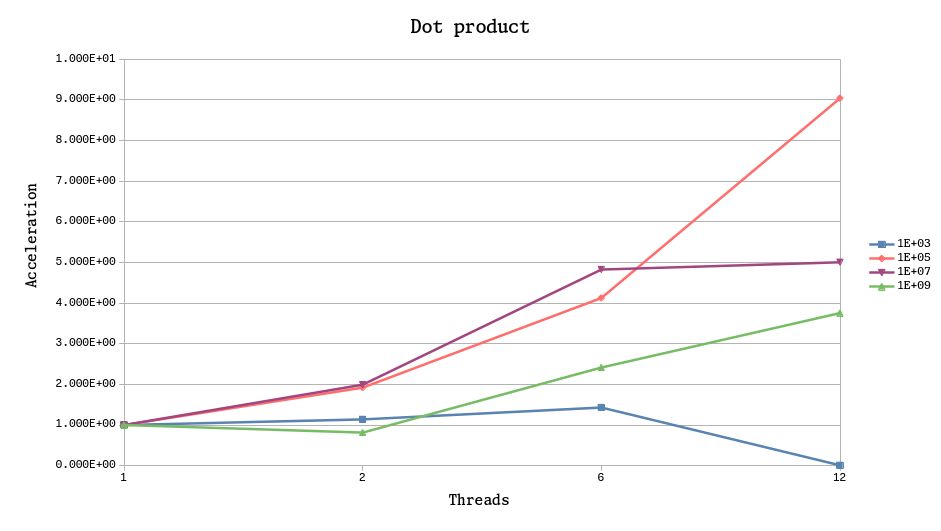
\includegraphics[scale=0.4]{dot-product} \\
При параллельном умножении векторов средних размерностей ($\approx \num{1e+5}$) получено ускорение
близкое к линейному. \\
\vspace{15mm}
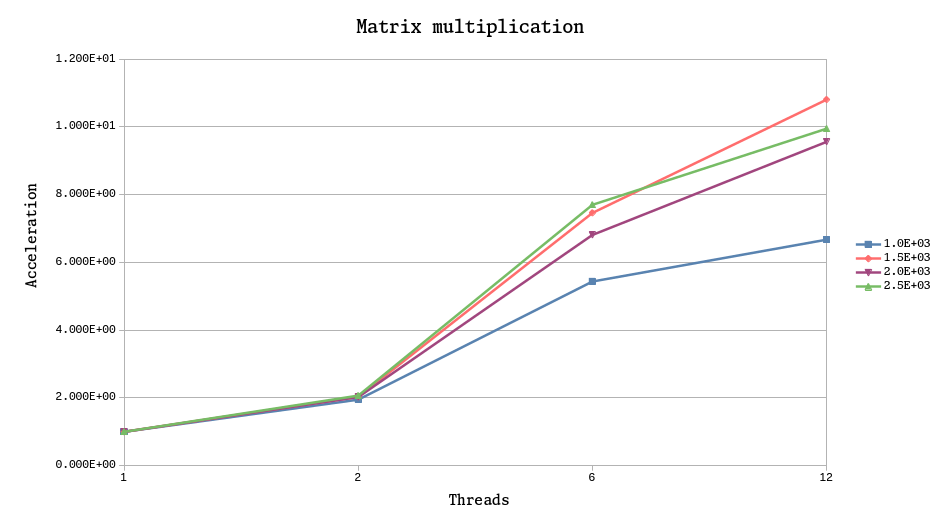
\includegraphics[scale=0.4]{mmlt}        \\
Ускорение, полученное при параллельном умножении матриц различной размерности, соответствует линейному. \\
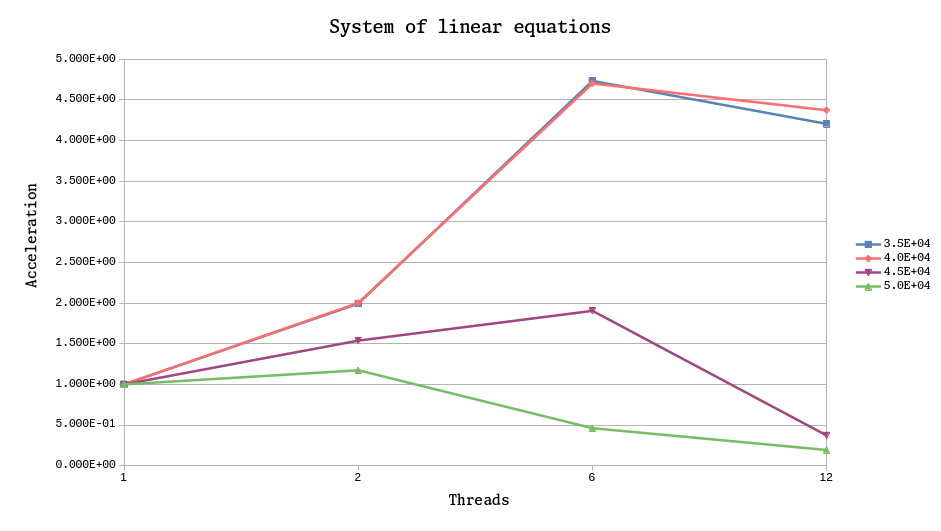
\includegraphics[scale=0.4]{sle}         \\
Параллельное решение СЛАУ с верхнетреугольной матрицей коэффициентов не привело к линейному ускорению.
\end{center}

\section{* Линейное комбинирование векторов}
\subsection{Постановка задачи}
Написать параллельную программу линейного комбинирования векторов:

$$ r = y + \alpha x $$

\noindentСравнить норму вектора результата при использовании различного числа потоков.

\subsection{Текст программы}
\begin{minted}{c}
void vec_cmb(struct vec* a, struct vec* b, struct vec* c, double k) {
#pragma omp parallel for num_threads(THRD)
  for (uint32_t i = 0; i < a->n; ++i)
    c->v[i] = a->v[i] + b->v[i] * k;
}

void vec_norm(struct vec* a, double* r) {
  double s = 0;

  for (uint32_t i = 0; i < a->n; ++i)
    s += a->v[i] * a->v[i];

  *r = sqrt(s);
}
\end{minted}
\textit{*вычислительные функции}

\begin{minted}{c}
int main() {
  ...

  struct vec* r = vec_new(N);
  struct vec* x = vec_seq(N);
  struct vec* y = vec_seq(N);

  double norm;
  double a = 3.0;

  clock_gettime(CLOCK_MONOTONIC, &s);
  vec_cmb(x, y, r, a);
  clock_gettime(CLOCK_MONOTONIC, &e);

  vec_norm(r, &norm);

  ...

  return 0;
}
\end{minted}
\textit{*вызывающая подпрограмма}

\begin{minted}{console}
[mehandes@pluto cmp]$ make
(0.0, 1.0, 2.0) + (0.0, 1.0, 2.0) * 3.0 = (0.0, 4.0, 8.0)
||r|| = 8.9442719
Execution time: 9.5580e-03 ms
\end{minted}
\textit{*результат выполнения при малой размерности векторов}

\newpage

\subsection{Результат выполнения}

\begin{table}[ht]
\centering
\begin{tblr}{
  width=\textwidth, 
  colspec={|l|X|X|}, 
  rowspec={|c|c|lllll|}
}
\SetCell[c=3]{c} $N = 10000$                                & & \\
Число потоков     & $||r||$               & $t, \unit{\ms}$     \\
1                 & 77593447.0244340      & 2.0349e+00          \\
2                 & 77593447.0244340      & 5.8907e-01          \\
4                 & 77593447.0244340      & 5.5830e-01          \\
8                 & 77593447.0244340      & 3.6830e-01          \\
12                & 77593447.0244340      & 7.6139e-01          \\
\end{tblr}
\end{table}

\end{document}

